\chapter{STP Tree Generator}
\label{stp_gen}
\section{Setup}
Our STP Tree Generator itself is made up of three different executables:
\begin{enumerate}
    \item The client uses the data from the received BPDUs and combines them into its path to the root.
    \item The server registers the clients and stores their information.
    \item The parser is used to obtain the finished visualization from the server.
\end{enumerate}
%TODO: rewrite this garbage
The intended way of using this tool is having multiple clients connect to a central server.
If there is a client connected to every bridge in the network, all of them will be in the report.
However, this does not mean that all connections are in the report as well, as connection information can only be obtained during tree buildup (see Section~\ref{packet_handling}).
An example setup can be seen in Figure~\ref{fig:example_setup}.

\begin{figure}[h]
    \centering
    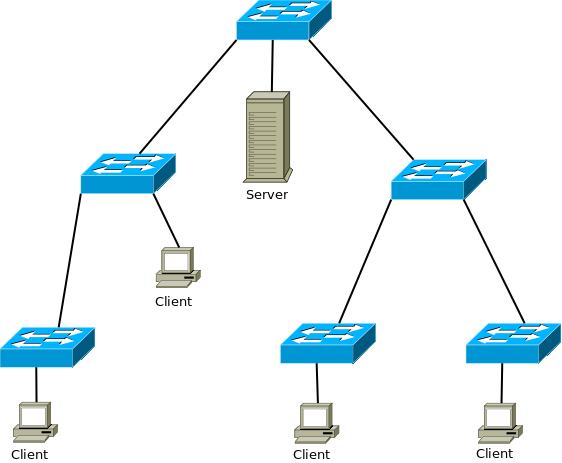
\includegraphics[width=0.7\textwidth]{example_setup.png}
    \caption{An example STP tree generator setup}
    \label{fig:example_setup}
\end{figure}

\section{Client-Server Communication}
For the communication we used Transmission Control Protocol (TCP) sockets.
TCP was used because it utilizes sessions, and takes care of guaranteeing correct transmission of the data.
An alternative would have been the User Datagram Protocol (UDP).
This would have slightly reduced the amount of network traffic.
It would however also have required us to implement some sort of message acknowledgement scheme, to ensure data is transmitted correctly.
There are three different message types in the packets we send:
\begin{enumerate}
    \item \textbf{register}: Clients send these message types to the server in order to receive an id.
    \item \textbf{push}: Clients send these message types when they push new tree information to the server.
    \item \textbf{report}: The parser sends this message type when requesting a visualization.
\end{enumerate}

Client ids are used in the server to differentiate information from different clients.
Once a push message with a certain client id is received, its contained data is stored along with the id.
If a message with the same id is received, this data is overwritten.
The clients take care of preserving and updating their respective information as necessary.
The timestamp for the last package, that a client sent to the server, is also associated with the id.

The server then uses these timestamps to identify and remove clients that are no longer connecting.
Path information pushed by these clients is also removed.
The timeout delay can be configured, as described in the section on configuration (Section~\ref{configuration}).
